\subsection{MVC}
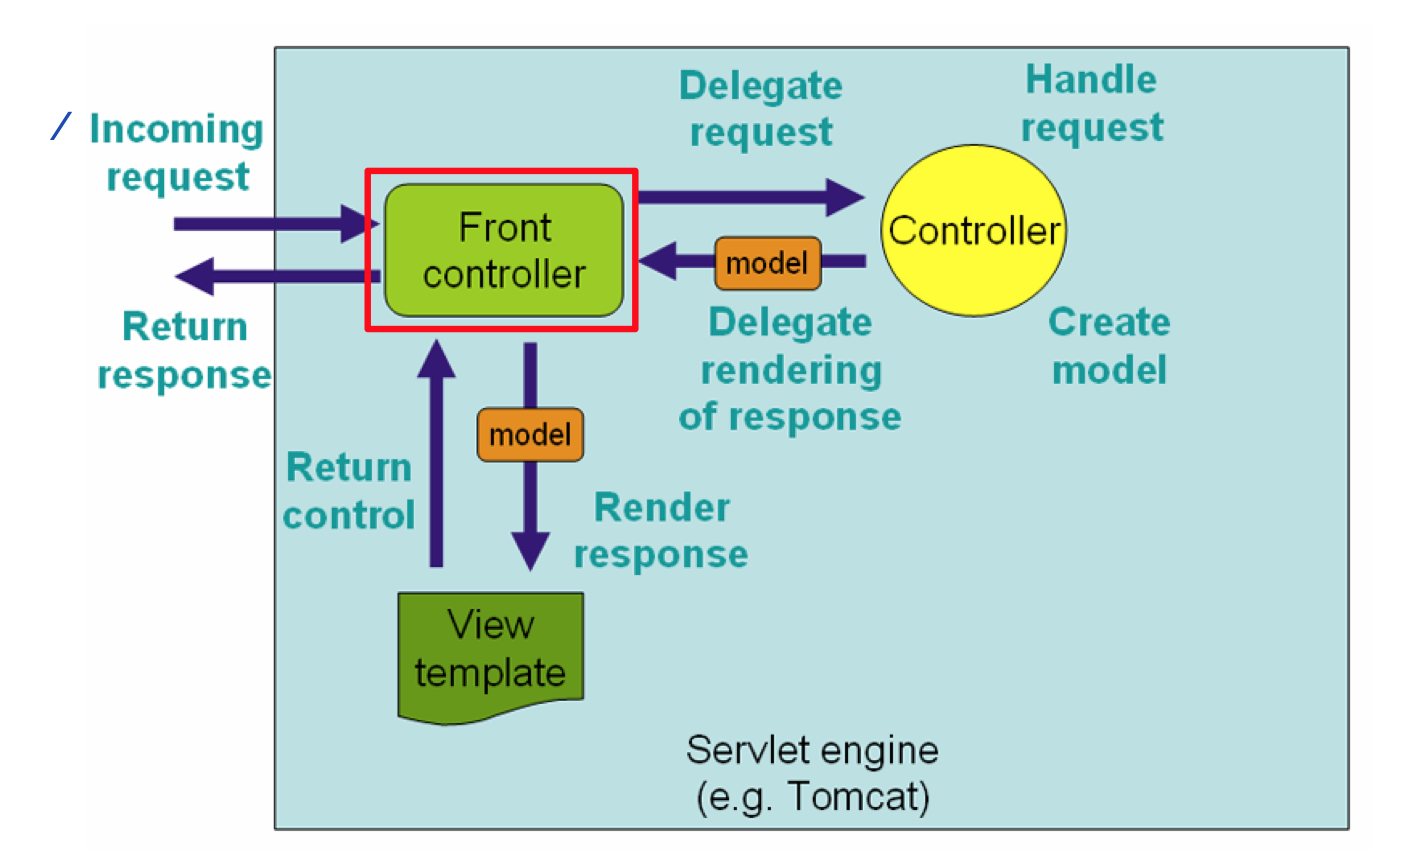
\includegraphics[width=\columnwidth]{images/mvcworkflow}
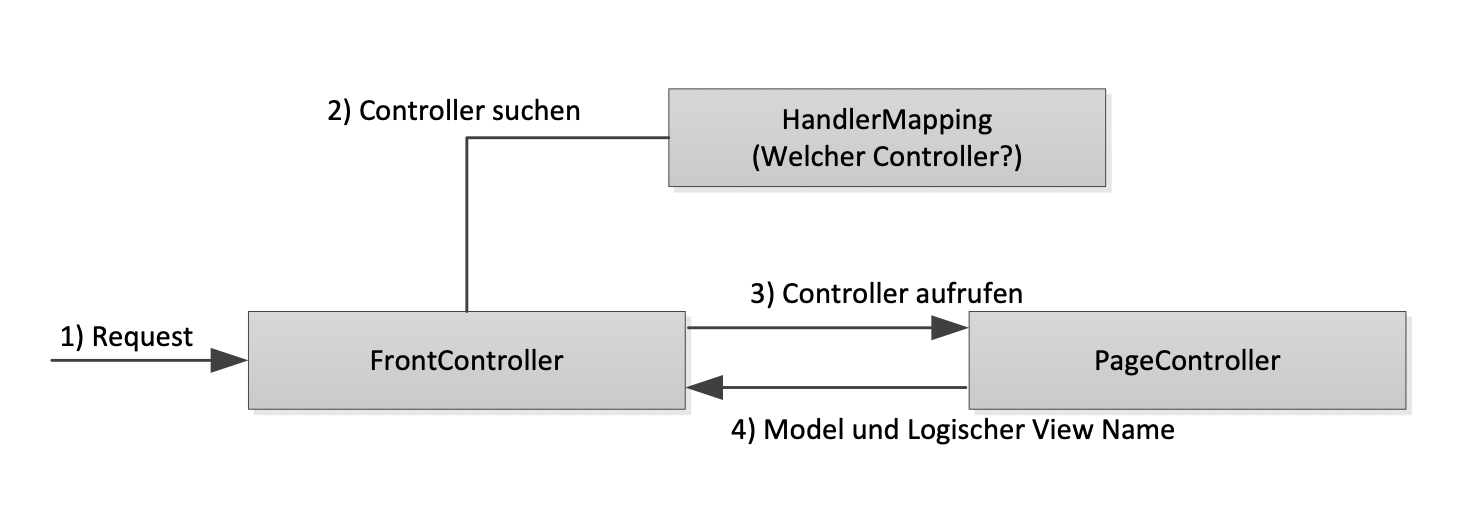
\includegraphics[width=\columnwidth]{images/algofrontpage}
\subsection{Front Controller}
Das «DispatcherServlet» wird bei jeder SpringMVC Applikation aufgrund der Annotationen \texttt{@SpringBootApplication} -> \texttt{@EnableAutoConfiguration} automatisch initialisiert. Das $«$DispatcherServlet$»$ wird per Default auf $"/"$ gemappt.

\begin{minted}[breaklines]{java}
@SpringBootApplication
@Slf4j
public class FlashcardApplication implements ApplicationRunner {
 
    @Autowired
    private QuestionnaireRepository questionnaireRepository;
 
    public static void main(String[] args) {
        SpringApplication.run(FlashcardApplication.class, args);
    }
}
\end{minted}
\begin{minted}[breaklines]{java}
@Controller
@RequestMapping("/questionnaires")
@Slf4j
public class QuestionnaireController {
 
    @Autowired
    private QuestionnaireRepository questionnaireRepository;
 
    @DeleteMapping("{id}")
    public ModelAndView delete(@PathVariable String id) {
        Optional<Questionnaire> questionnaire = questionnaireRepository.findById(id);
        if (questionnaire.isPresent()) {
            questionnaireRepository.deleteById(id);
            return new ModelAndView("redirect:/questionnaires");
        } else {
            return new ModelAndView("404");
        }
    }
 
    @PostMapping()
    public ModelAndView create(@Valid Questionnaire questionnaire, BindingResult result) {
        if (result.hasErrors()) {
            log.error("Validation Errors: {}", result.getAllErrors());
            ModelAndView modelAndView = new ModelAndView("create");
            modelAndView.addObject("questionnaire", questionnaire);
            return modelAndView;
        }
        log.debug("Create Questionnaire: {}", questionnaire);
        questionnaireRepository.save(questionnaire);
        log.debug("Questionnaire persisted: {}", questionnaire);
        return new ModelAndView("redirect:/questionnaires");
    }
 
    @GetMapping(params = "form")
    public ModelAndView getCreateForm() {
        ModelAndView modelAndView = new ModelAndView("create");
        modelAndView.addObject("questionnaire", new Questionnaire());
        log.debug("Call view 'create'");
        return modelAndView;
    }
 
    @GetMapping("update/{id}")
    public ModelAndView getUpdateForm(@PathVariable String id) {
        Optional<Questionnaire> questionnaire = questionnaireRepository.findById(id);
        if (!questionnaire.isPresent()) {
            return new ModelAndView("404");
        }
        ModelAndView modelAndView = new ModelAndView("update");
        modelAndView.addObject("questionnaire", questionnaire.get());
        log.debug("Call view 'update'");
        return modelAndView;
    }
 
    @PutMapping()
    public ModelAndView update(@Valid Questionnaire questionnaire, BindingResult result) {
        if (result.hasErrors()) {
            log.error("Validation Errors: {}", result.getAllErrors());
            ModelAndView modelAndView = new ModelAndView("update");
            modelAndView.addObject("questionnaire", questionnaire);
            return modelAndView;
        }
        log.debug("Update Questionnaire: {}", questionnaire);
        questionnaireRepository.save(questionnaire);
        log.debug("Questionnaire persisted: {}", questionnaire);
        return new ModelAndView("redirect:/questionnaires");
    }
 
    @GetMapping
    public String findAll(Model model) {
        List<Questionnaire> questionnaires = questionnaireRepository.findAll();
        log.debug("{} questionnaires found", questionnaires.size());
        model.addAttribute("questionnaires", questionnaires);
        return "list";
    }
 
    @GetMapping(value = "/{id}")
    public String findById(@PathVariable String id, Model model) {
        log.debug("find questionnaire by id {}", id);
        Optional<Questionnaire> questionnaire = questionnaireRepository.findById(id);
        if (questionnaire.isPresent()) {
            model.addAttribute("questionnaire", questionnaire.get());
            log.debug("found questionnaire {}", id);
            return "show";
        } else {
            log.debug("no questionnaire found");
            return "404";
        }
    }
}
\end{minted}